\chapter{Návrh a testovanie softvéru}
\label{tests_design}
Kapitola popisuje vývoj softvéru so zameraním na testovanie. 
Prvá časť kapitoly približuje životný cyklus vývoja softvéru, druhá sa venuje overovanie správnosti softvéru, tretia štvrtá metódam a úrovniam testovania.

\section{Modely životného cyklu softvéru}
\label{life_cycles}
Vývoj softvéru je možné rozdeliť do niekoľkých častí, pričom každá z nich rieši iné problémy a na konci sú výsledky, ktoré je možné overiť.
Nie každý model implementuje všetky tieto etapy a v niektorých modeloch sa zase naopak určité časti opakujú viackrát.
\begin{itemize}
	\item \textbf{Plánovanie} - Konceptuálny návrh a plánovanie
	\item \textbf{Analýza} - Zhromažďovanie požiadavok a ich analýza
	\item \textbf{Návrh} - Návrh architektúry a špecifikácii
	\item \textbf{Vývoj} - Testovanie, implementácia
\end{itemize}

\section*{Vodopádový model}
\label{waterfall_model}
Prvý formálne popísaný a asi najznámejší model životného cyklu softvéru~\ref{waterfall_model_fig}.
Bol prezentovaný už v~roku 1970 a vyjadruje postupnosť fáz: získavanie požiadavok, systémová analýza, programovanie, testovanie, implementácia a údržba systému.
Často používaný prí výučbe, je jednoduchý a ľahko sa vysvetľuje.
Definuje a plánuje fázy, čím pomáha dodržovať termíny a výstupy jednotlivých fáz, ale je veľmi málo flexibilný, keďže počíta stým, že požiadavky sa nebudú meniť, takže plánovanie všetkých úloh projektu je treba naplánovať do posledného detaily, čo je náročné a drahé~\cite{Patton}.
\begin{figure}[H]
\centering
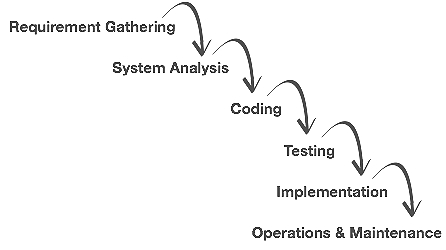
\includegraphics[width=0.65\linewidth]{obrazky/waterfall_model.png}
\caption{Vodopádový model~\cite{models}}
\label{waterfall_model_fig}
\end{figure}

\section*{V~model}
\label{v_model}
Podobný vodopádovému modelu~\ref{waterfall_model}, no každá fáza pred programovaním má k~sebe doplnkovú fázu, ktorá overuje výsledky fázy pred programovaním~\ref{v_model_fig}.
Napríklad keď sú stanovené požiadavky na softvér, tak hneď môžu byť napísané akceptačné testy~\ref{acceptance_tests}.
No reálne overenie môže nastať až keď je softvér implementovaný.
V tomto modely je použitých niekoľko testovacích techník, pričom každá z~nich overuje inú časť návrhu, designu, alebo implementácie~\cite{Patton}.
\begin{figure}[H]
\centering
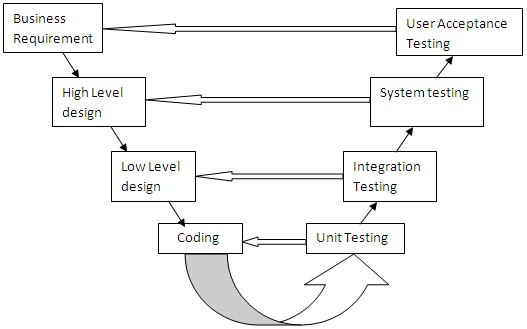
\includegraphics[width=0.65\linewidth]{obrazky/v_model.png}
\caption{V~model~\cite{models}}
\label{v_model_fig}
\end{figure}

Testovanie softvéru je aktivita, ktorá pomáha vyhodnocovať, či chovanie systému zodpovedá tomu, čo je pre neho definované.
Proces testovania pomáha tvorcom softvéru vyhodnotiť, ktoré časti sa správajú správne a ktoré nie, čiže identifikuje chyby v~programe.
Chyby môžu vznikať z~rôznych príčin, no všeobecne platí, že čím skôr sa chyba odhalí, tým ľahšie a teda aj lacnejšie je opraviteľná.
Testovanie je súčasťou verifikácie systému, ktorá je zase súčasťou procesu zabezpečovania kvality softvéru (Quality Assurance, QA).~\cite{hornicky}

\section{Verifikácia a validácia}
Tieto 2 pojmy sú často zamieňané, alebo považované za synonymá.
Aj keď obidva pojmy slúžia na zvyšovanie kvality softvéru, každý z~nich znamená niečo iné.
Verifikácia overuje, či softvér spĺňa technickú špecifikáciu, čiže úlohu na ktorú bol navrhnutý.
\textbf{Verifikovať} sa dá viacerými postupmi:
\begin{itemize}
	\item \textbf{Statická analýza} skúma vlastnosti softvéru bez jeho spúšťania.
	\item \textbf{Dynamická analýza} overuje vlastnosti softvéru práve jeho spúšťaním.
	\item \textbf{Formálna verifikácia} pomocou formálnych metôd overuje, že systém odpovedá špecifikácii.
	\item \textbf{Testovanie} skúma softvér spúšťaním programu za účelom zvýšenia jeho kvality.
\end{itemize}

\textbf{Validácia} potvrdzuje, že softvér spĺňa obchodné podmienky a požiadavky používateľa, nie technickú špecifikáciu.

\section{Metódy testovania softvéru}
Pri návrhu testov je veľmi dôležité do akej miery tester pozná vnútornú štruktúru systému.
Ak sa podieľal na vývoji a dobre ho pozná bude testy navrhovať úplne iným spôsobom ako osoba, ktorá môže mať skúsenosti s~testovaním, no systém nepozná.
Táto kapitola ďalej rozoberá rozdiely v~testovaní pri rozdielnych znalostiach o~systéme.

\subsection*{Testovanie čiernej skrinky vs. testovanie bielej skrinky}
\label{blackbox_vs_whitebox}
Pri testovaní metódou \textbf{čiernej skrinky} sa softvér považuje za nepriehľadnú skrinku a tester nemá žiadne informácie o~jej vnútornej štruktúre.
Má informácie o~úlohe softvéru, ale nie o~spôsobe vykonávania tejto úlohy.
Pri tejto metóde je dôležité poznať vlastnosti množiny vstupných dát a vybrať z~nich podmnožinu, ktorá otestuje čo najväčšiu časť možných prípadov.
Tento prístup je výhodný pri odhaľovaní chýb v~špecifikácii.
Metóda sa používa pri akceptačnom aj regresnom testovaní.

\textbf{Testovanie bielej skrinky} je naopak postavené na fakte, že tester pozná vnútornú štruktúru softvéru.
K~takémuto testovanie je potrebný zdrojový kód, alebo pseudokód popisujúci chovanie softvéru.
Tým, že tester presne pozná štruktúru softvéru dokáže lepšie odhadnúť chovanie systému a pri výbere testovacích prípadov môže voliť napríklad také testovacie prípady aby boli pri testovaní použité všetky vetvy kódu.

Existuje prístup kombinujúci testovanie čiernej a testovanie bielej skrinky, \textbf{testovanie šedej skrinky}.
Tester pozná vnútorné dátové šktruktúry a algoritmy, ale nepozná reálnu imlplementáciu, čiže nedokáže navrhovať testy s~ohľadom na pokrytie kódu.
Tento prístup je čím ďalej, tým viac používaný hlavne kvôli zjednodušeniu návrhu testov bez nutnosti sa podrobne vyznať v~implementácii.

\section{Úrovne testovania softvéru}
\label{testing_levels}
Ako ukazujú modely životného cyklu softvéru, rôzne časti (úrovne) systému je možné testovať pri rôznych príležitostiach. 
Nedá sa testovať stále a všetko, je potrebné určiť kedy budú ktoré časti testované.

\subsection*{Jednotkové testy}
\label{unit_tests}
Jednotkové testy (Unit tests) pracujú iba s~jednou jednotkou(komponentom, modulom), ktorú testujú.
Preto sa im niekedy hovorí aj testovanie komponent (Component testing), alebo testovanie modulov (Module testing).
Jednotka by mala byť čo najmenšia, ale dostatočne veľká, aby bola samostatne testovateľná.
Tieto testy sú často robené priamo programátormi a chyby sú odstraňované ihneď ako je to možné.

\subsection*{Integračné testy}
\label{integration_tests}
Integračné testy overujú funkčnosť rozhrania medzi komponentami, ktoré môžu byť malé ako pri jednotkových testoch a postupne s~vývojom softvéru sa zväčšovať až sa testuje integrácia celého podsystému do už používaného systému.
Tento prístup sa nazýva inkrementálne integrovanie a chyby dokáže odhaliť pomerne skoro, no je drahý, keďže sa musia simulovať rozhrania, ktoré ešte neboli implementované.
Opačný prístup k~integračný testom sa nazýva integrácia veľkým treskom a testuje sa až keď sú všetky súčasti systému implementované.
Tento prístup je rýchly a jednoduchý, no je náročne zistiť príčinu zlyhania takejto neskorej integrácie.
Ideálny prístup je niekde medzi týmito dvoma extrémnimy prípadmi.
Testovať väčšie súčasti, ktoré by mohli spôsobovať problémy.

\subsection*{Systémové testy}
\label{system_tests}
Systémové testy sú robené na takmer hotovom sofvéry a je u~nich vyžadovaná nezávislosť, takže ich robia viaceré tými alebo tretia strana.
Cieľom systémových testov je overiť, že softvér spĺňa špecifikáciu.

\subsection*{Akceptačné testy}
\label{acceptance_tests}
Akceptačné testy sú narozdiel od ostatných typov testov zodpovednosťou zákazníka, keďže overujú, či softvér spĺňa požiadavky zákazníka a či je pripravený na prevádzku.
Hľadanie chýb nie je primárnou úlohou akceptačných testov.

\subsection*{Regresné testovanie}
\label{regression_tests}
Regresné testy sú robené stále, ak sa zmení nejaká časť softvéru na zaistenie, že nová verzia zdieľa vlastnosti starej a že sa do systému nezaniesli nové chyby.
Toto testovanie prebieha často, takže regresné testy sú veľakrát automatizované.

\section{Automatizácia testov}
\label{tests_automatization}
Testovanie je časovo a finančne náročná činnosť, preto je dobré ho čo najviac automatizovať.
Napríklad ak by sa mal manuálne testovať celý systém po každom vydaní novej verzie, ktorá len opravuje chyby starších verzií, bola by to sizyfovská práca.
No nie všetko testovanie sa dá automatizovať, čo môže byť aj dobre.
Ak automatické testy minú chybu pri prvom spustení, tak tú chybu budú míňať pri každom ďalšom testovaní.
Chyba sa stane imúnna voči testom.

\section{Pojmy z testovania}
\label{pojmy_testovanie}
V nasledujúcich kapitolách sa venujú testovania a tvorbe testvacích sád na praktickejšej úrovni a sú tam používané pojmy z testovania, preto je vhodné tieto pojmy vysvetliť.
V testovaní, ako aj v iných oblastiach je možné jeden pojem definovať viacerými názvami, takže nasledujúce pomenovania sú vysvetlené v kontexte tejto práce~\cite{Smrcka}.

\begin{description}
	\item[Test case (testovací prípad)] \hfill \\
		Testovací prípad sa skladá zo vstupných hodnôt, očakávaných výsledkov a tiež z prefixových a postfixových hodnôt( pre prípravu progrmau pred testom a jeho vyčistenie po teste).

	\item[Test set / test suite (testovacia sada)] \hfill \\
		Testovacia sada je množina testovacích prípadov.

	\item[Test requirement (požiadavok na test)] \hfill \\
		Požiadavok na test je špecifický element softvéru, ktorý musí daný test pokryť, alebo splniť: 
		\begin{itemize}
			\item riadok kódu, 
			\item vetvenie kódu, 
			\item konkrétna trieda, 
			\item konkrétna správa posielaná objektom, \dots
		\end{itemize}

	\item[Softvérový artefakt] \hfill \\
		Softvérový arefakt je subjekt programátora pomocie neho tvorí výsledný produkt, napríklad: 
		\begin{itemize}
			\item \texttt{časti kódu} (moduly, triedy, metódy, funkcie), 
			\item \texttt{riadky kódu} (príkaz, volaná funkcia, usporiadnanie paramterov), 
			\item \texttt{riadiaca logika} (cykly, podmienky, logicke výrazy, podmienky), 
			\item \texttt{práca s datami} (premenné, dátové typy, konštatny, operátory, pretypovanie), 
			\item \texttt{logika behu} (usporiadanie sekvencií volaní, atomicita operácii, synchronizčné primitíva), 
			\item \texttt{predpoklady prostredia} (výkon stroja, verzia knižníc, premenné prostredie, konfigurácia OS, sieťové pripojenie a jeho kvalita), 
			\item \texttt{kombinácia softvérových artefaktov}, \dots
		\end{itemize}

	\item[System under test (SUT)] \hfill \\
		Testovaný systém, alebo iná entita (modul, trieda, \dots), ktorá je testovaná.

	\item[Coverage (pokrytie)] \hfill \\
		Pokrytie je miera udávajúcia ako veľmi daná testovacia sada skúma testovaný systém (SUT). Pri testovaní sofvéru sa používa code coverage. Typicky sa udáva sa v percentách, vzťahuje sa k danému kritériu pokrytia a k danej testovacej sade.

	\item[Coverage criterion (kritérium pokrytia)] \hfill \\
		Kritérium pokrytia je pravidlo, alebo predpis pre systematické generovanie požiadavkov na testy.
\end{description}

